\labwork{Установка IDE \eclipse}\label{eclipseinstall}

\bigskip
Для работы IDE \eclipse\ требуется установленная Java \labref{javainstall}.

\bigskip
Для установки доступны два варианта:
\begin{enumerate}
\item \textbf{Eclipse Standard} базовый вариант среды, в ЛР рассмотрен именно он для иллюстрации 
ручной установки расширений
\item \textbf{Eclipse IDE for C/C++ Developers} вариант сборки 
уже включает расширение CDT, поэтому в следующий раз рекомендуем сразу качать его,
это упростит и съэкономит немного времени на установку рабочей среды
\end{enumerate}

\bigskip\wcmd{\url{http://www.eclipse.org/downloads/}}

\bigskip\menu{Eclipse Standard>Windows 32
Bit>Download>\file{eclipse-standard-luna-R-win32.zip}}

\bigskip Перетащите каталог \file{eclipse} из архива в \file{D:/ARM} и
создайте удобным для вас способом ссылку на \file{D:/ARM/eclipse/eclipse.exe}.

\bigskip
\includegraphics[height=0.3\textheight]{eclipse/EclipseSplash.png}

\bigskip Workspace\ --- рабочий каталог, в котором создаются каталоги отдельных
проектов, типа \file{D:/WORK}. Eclipse создаст в нем служебный каталог
\file{.metadata}, и поместит в него служебную информацию, относящуюся сразу ко
всем проектам. Как побочный эффект, если в workspace уже есть какой-то каталог,
можно создать новый проект (например \file{book}), и в левой части рабочей
области \eclipse\ в окне \window{Project Explorer}\ появится дерево файлов
\file{book/*}.

\bigskip\menu{\file{D:/ARM/eclipse/eclipse.exe}>Workspace>\file{D:/ARM}>Use as
default>OK}

\bigskip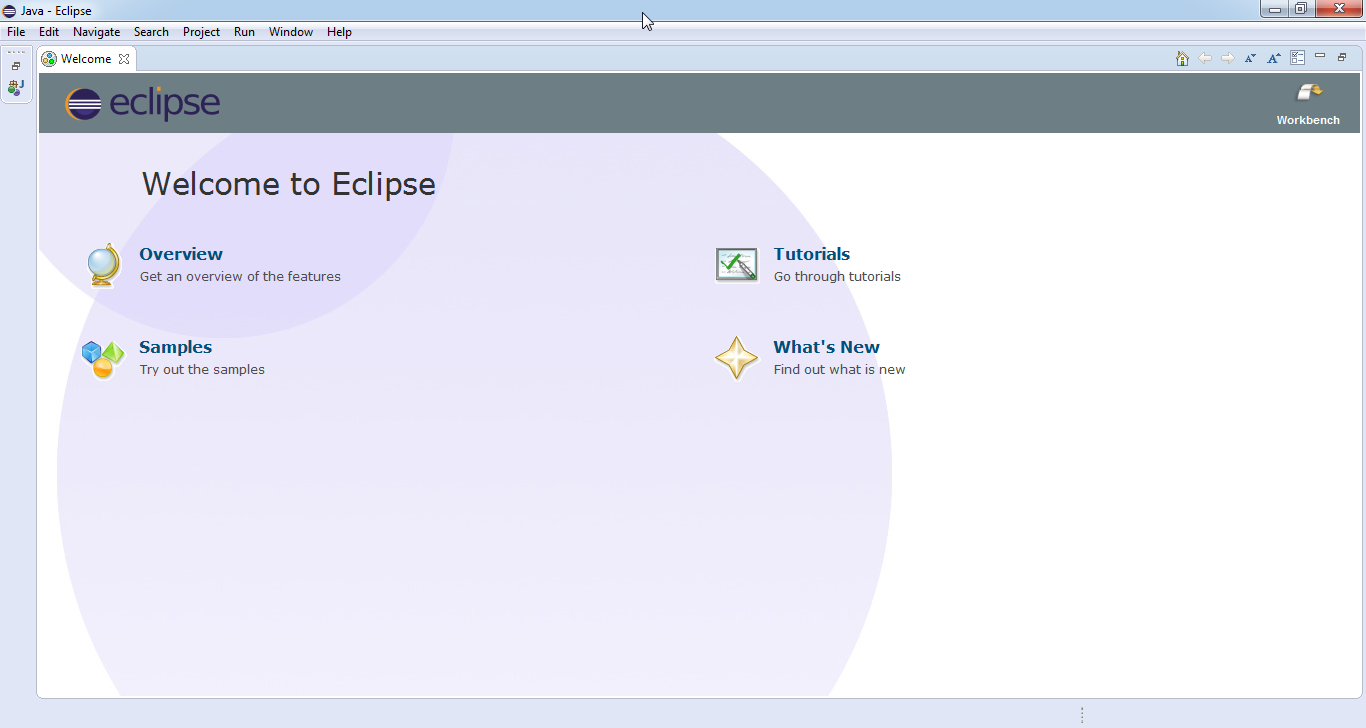
\includegraphics[width=0.9\textwidth]{eclipse/EclipseMain.png}

\bigskip Проверяем наличие обновлений

\bigskip\menu{Help>Check for Updates>Details>No updates found>OK}

\bigskip В базовом варианте Eclipse поддерживает только Java, поэтому нужно
установить расширение для работы с С/C++: \file{CDT}.

\bigskip
Проект \file{CDT}\ предоставляет полнофункциональную интегрированную среду
для разработки на Си и \cpp. Поддерживаются: управление проектами и
компиляцией для различных тулчейнов, стандартная сборка через
\file{make}, навигация по исходным текстам, различные инструменты для
работы с иходным текстом, такие как иерархия типов, граф вызовов, браузер
подключаемых файлов, браузер макроопределений, редактор кода с подсветкой
синтаксиса, сворачивание синтаксических структур (фолдинг) и гипертекстовая
навигация, рефакторинг и генерация кода, средства визуальной отладки,
включающие просмотр памяти, регистров и дизассемблер.

\bigskip\wcmd{\url{http://www.eclipse.org/cdt/downloads.php}}

\bigskip Выделить и скопировать в буфер обмена ссылку

\file{p2 software repository}:
\url{http://download.eclipse.org/tools/cdt/releases/8.4}.

\bigskip Добавляем сетевое хранилище пакетов для \eclipse:

\bigskip\menu{\eclipse>Help>Install New Software>Work with>Add}

\bigskip\menu{Name>CDT}

\menu{Location>http://download.eclipse.org/tools/cdt/releases/8.4}

\menu{OK}

\bigskip
Выбрать (если оно не выбралось само) хранилище \menu{Work with:>CDT},
и в дереве выбора пакетов выбрать:

\bigskip
\dirtree{%
.1 CDT.
.2 CDT Main Features.
.3 \checkbox\ C/C++ Development Tools.
.2 CDT Optional Features.
.3 \checkbox\ C/C++ C99 LR Parser.
.3 \checkbox\ C/C++ GCC Cross Compiler Support.
.3 \checkbox\ C/C++ GDB Hardware Debugging.
}

\bigskip
\menu{Next>Next>Licenses>Accept>Finish}

\bigskip После установки пакетов появится окно с запросом перезапуска \eclipse.

\bigskip Аналогично ставим плагин GNU ARM Eclipse:

\bigskip
\menu{Help>Install>Work with>Add}

\menu{Name>GNU ARM plugin}

\menu{Location>\url{http://sourceforge.net/projects/gnuarmeclipse/files/Eclipse/updates/}}

\dirtree{%}
.1 GNU ARM C/C++ Cross Development Tools.
.2 \checkbox\ Cross Compiler Support.
.2 \checkbox\ Generic Cortex-M Project Template.
.2 \checkbox\ STM32Fx Project Templates.
.2 \checkbox\ OpenOCD Debugging Support.
}

\menu{Warning: You install unsigned content>Ok}

\bigskip
В \eclipse\ есть так называемые \term{перспективы} (perspective)\ --- это
переключаемые режимы отображения рабочего набора окон, настроенные под тип
работы. По умолчанию запускается перспектива \window{Java}. Нас
интересует перспектива \window{C/C++}:

\bigskip\menu{Window>Open Perspective>Other>C/C++>Ok}

\bigskip Также перспективу можно переключить кнопкой на панели в правом верхнем
углу:

\bigskip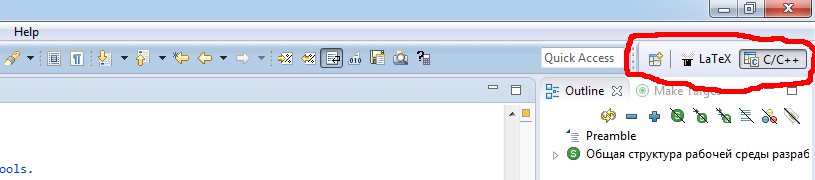
\includegraphics[width=0.9\textwidth]{eclipse/eclperpective.png}

\bigskip Для настройки привычных вам клавиш можно сразу зайти в
глобальные настроки среды и поменять привязку клавиш:

\bigskip\menu{Window>Preferences>General>Keys}

\menu{Type filter here:>F12}

\menu{Command}

\menu{Activate Editor>Binding>/удалить/}

\menu{Build Project>Binding>/нажать \keys{F12}/}

\menu{Apply>OK}


